\documentclass[12pt]{article}
\usepackage{../../../lecture_notes}
\usepackage{../../../math}
\usepackage{../../../uark_colors}

\hypersetup{
  colorlinks = true,
  allcolors = ozark_mountains,
  breaklinks = true,
  bookmarksopen = true
}

\newcommand{\answer}[1]{{\color{blue_winged_teal}\textbf{Answer:} #1}}
\newcommand{\pts}[1]{{\color{zinc500}#1}}

\begin{document}
\begin{center}
  {\Huge\bf Midterm 1 - Fall 2024}
  
  \smallskip
  {\large\it  ECON 4753 — University of Arkansas}
\end{center}

\vspace{5mm}
\begin{enumerate}
  \item \pts{(15pt)} Say you have a sample of 100 companies where you observe the average wage and the number of non-managerial employees. You regress the $\log$ of average wage at a company on the number of non-managerial employees and estimate a coefficient of $\hat{\beta}_1 = 0.005$. Interpret this coefficient estimate in words.
  
  \answer{The estimated coefficient suggest that a firm with one additional employee is predicted to pay a 0.5\% higher average wage. ($\log$ is interpreted as a percent change)}



  \vspace{5mm}
  \item Below is a graph using data from law schools. Along the X axis is the rank of the law school (1 is best) and along the Y axis is the median starting salary for graduates. On the chart, I have ploted estimates from a linear regression of $Y$ on $X$ and a fourth-order polynomial of $X$.
  \begin{enumerate}
    \item \pts{(10pt)} How would I evaluate which model performs `better' on this sample?
    
    \answer{I would estimate the in-sample mean-squared prediction error and whichever model had a lower MSPE would perform `better'}

    \item \pts{(10pt)} Describe which of the two models you would use if your goal is predicting median starting salary given the rank of a law school? 
    
    \answer{Since the fourth-order polynomial line (in yellow) fits the data better, it would be prefereable for prediction in this case. It does not seem to be overfitting the data.}

    \item \pts{(10pt)} Why might someone want to use the linear model in this context?
    
    \answer{In this context, the linear model is less accurate at prediction but is easier to explain (i.e. for every 10-unit descrease in school rank, we predict a median starting salary decrease of $10 \hat{\beta}_1$.)}
  \end{enumerate}

  \begin{center}
    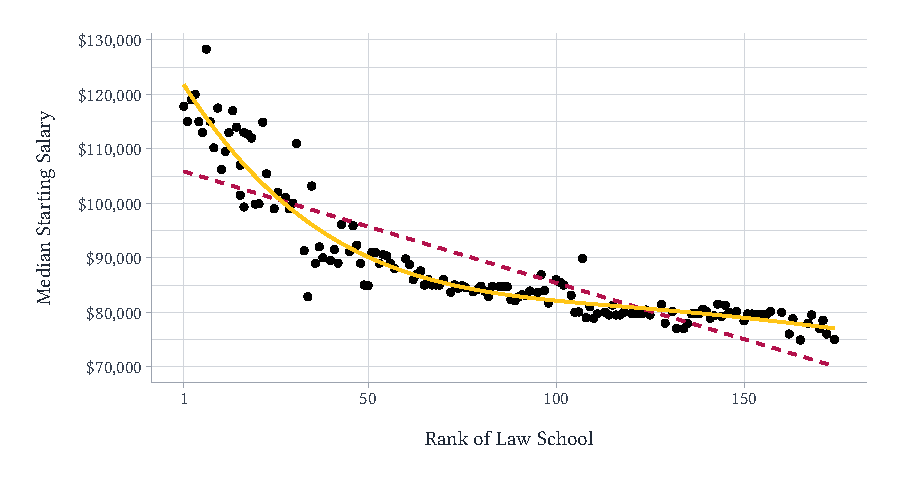
\includegraphics[width = 0.85\textwidth]{figures/plot_law_school_rank_and_salary.pdf}
  \end{center}





  \vspace{5mm}
  \item Continuing with the law school example, say we regress salary on an intercept and an indicator being a top 25 ranked program (=1 if ranked in top 25, =0 otherwise). We estimate a coefficient of 27177 and a standard error of 1528. 
  \begin{enumerate}
    \item \pts{(15pt)} Can you reject the null that top 25 ranked law schools do not earn more than other law schools?
    
    \answer{The confidence interval is $27177 \pm 1.96 * 1528 = (24182, 30171)$. Since this confidence interval does not contain $0$, we can reject the null that a school ranked in the top 25 does not have a statistically significantlly different median starting salary.}
  \end{enumerate}




  \vspace{5mm}
  \item Continuing with the law school example, the regression model estimate is as follows: 
  \begin{codeblock}[{}]
OLS estimation, Dep. Var.: salary
               Estimate  Std. Error   t value   Pr(>|t|)    
(Intercept)  106063.518   1405.0819   75.4856  < 2.2e-16 ***
rank           -206.731     12.5843  -16.4278  < 2.2e-16 ***
---
Signif. codes:  0 '***' 0.001 '**' 0.01 '*' 0.05 '.' 0.1 ' ' 1
  \end{codeblock}

  \begin{enumerate}
    \item \pts{(10pt)} Interpret the coefficient on a law school's \texttt{rank}
    
    \answer{A school with a rank of 10 schools lower, we predict their median starting salary to be $-\$2060$ lower. (1 school lower predicts a $-\$206$ lower). This estiamte is statistically significantly different from 0.}
    
    \item \pts{(10pt)} Form a 95\% confidence interval for the rank coefficient (the critical value of the middle 95\% is $\pm 1.96$).
    
    \answer{With 95\% confidence, we think the true association of rank and median starting salary is within this range $-206.731 \pm 12.5843 = (182.06, 231.39)$.}
  \end{enumerate}
  



  \vspace{5mm}
  \item Continuing with the law school example, schools can be broken up into 4 US regions: Northeast, South, Midwest, and the West. We want to see if different regions have different starting salaries. We regress median starting salaries on dummies for each region (excluding one)
  \begin{codeblock}[{}]
OLS estimation, Dep. Var.: salary
                    Estimate Std. Error   t value  Pr(>|t|)    
(Intercept)        88366.52    2143.09 41.233212 < 2.2e-16 ***
region::Northeast   3874.39    3097.83  1.250681   0.21308    
region::South      -4025.82    2499.87 -1.610412   0.10950    
region::West        1568.09    2828.93  0.554307   0.58023    
---
Signif. codes:  0 '***' 0.001 '**' 0.01 '*' 0.05 '.' 0.1 ' ' 1
  \end{codeblock}

  \begin{enumerate}
    \item \pts{(10pt)} What is the omitted group in this case?

    \answer{The omitted group is the Midwest.}

    \item \pts{(10pt)} What is the average median starting salary for lawyers who went to school in the West? 
    
    \answer{The average median starting salary for lawyers in the west is $88366.52 + 1568.09 = 89934.61$.}
  \end{enumerate}

\end{enumerate}



\end{document}
